\documentclass[conference]{IEEEtran}
\usepackage[utf8]{inputenc}
\usepackage[T1]{fontenc}
\usepackage{graphicx} % Required for including images
\usepackage{lipsum} % Provides dummy text
\usepackage{amsmath} % Required for \sqrt and other math commands
\usepackage{xcolor}

\definecolor{myblue}{HTML}{717AFD}
\definecolor{myred}{HTML}{F0564A}
\definecolor{mygrey}{HTML}{464546}

\setlength{\parskip}{0.8em}  % Adjust the value to your liking, e.g., 1em, 12pt, etc.

\newcommand\wordcount{
   \immediate\write18{wordcount.bat \jobname.tex}
   \input{\jobname.wc}
}

\newcounter{totalfigures}
\setcounter{totalfigures}{0}
\let\oldfigure\figure
\def\figure{\stepcounter{totalfigures}\oldfigure}

\begin{document}

\title{Laboratory Exercise in Electromyography}
\author{Blind grading number 2504F}
\maketitle

\begin{abstract}
This report provides a comprehensive analysis of surface electromyography (sEMG), focusing on the effects of electrode orientation and size on signal quality. 
Unexpected results from the parallel versus perpendicular electrode experiment highlighted the necessity of internal data quality control,
 particularly in managing 50Hz noise. Experiments with different electrode sizes revealed an inverse relationship between spatial resolution 
 and signal quality, emphasizing the need for careful calibration and real-time processing algorithms. The report also suggests the potential 
 for improved prosthetic control through the use of an increased number of smaller electrodes. Overall, the findings contribute to a better understanding of sEMG 
 measurements and the factors involved in generating a higher quality signal.
\end{abstract}

\section{Introduction}
Electromyography (EMG) is a versatile biomedical tool for non-invasively monitoring, recording, and 
analyzing myoelectric signals from muscle fibers \cite{farinaInterpretationSurfaceElectromyogram2006}. These signals reveal crucial information 
about muscle behavior, abnormalities, and functional states. EMG operates through various methodologies, with 
surface EMG (sEMG) being a focal point due to its non-invasive nature, despite some limitations in spatial 
resolution and signal quality (Fig. \ref{fig:actionpotential}).

This report concentrates on kinesiological EMG, specifically the neuromuscular activation during different 
movements using sEMG. The captured myoelectric signals provide insights into muscle 
condition and characteristics, such as fatigue and strength, through variations in signal patterns. The ability 
of sEMG to record from a broad area, although resulting in signal superposition from surrounding 
muscles, allows for detailed analysis and identification of specific muscle activations with 
advanced signal processing techniques \cite{phinyomarkFeatureReductionSelection2012}.

EMG finds extensive applications in medical research, sports science, rehabilitation, and ergonomics, 
contributing to enhanced understanding of muscle movements, development of specialized equipment, and 
improvement in product design. 

In summary, this report aims to explore the detailed aspects of EMG, with a focus on sEMG, its applications, 
and the challenges associated with correlating EMG signals to muscle behavior, as well as its use as a source 
of data to drive the movement of artificial prostheses.

\begin{figure}[h]
   \centering
   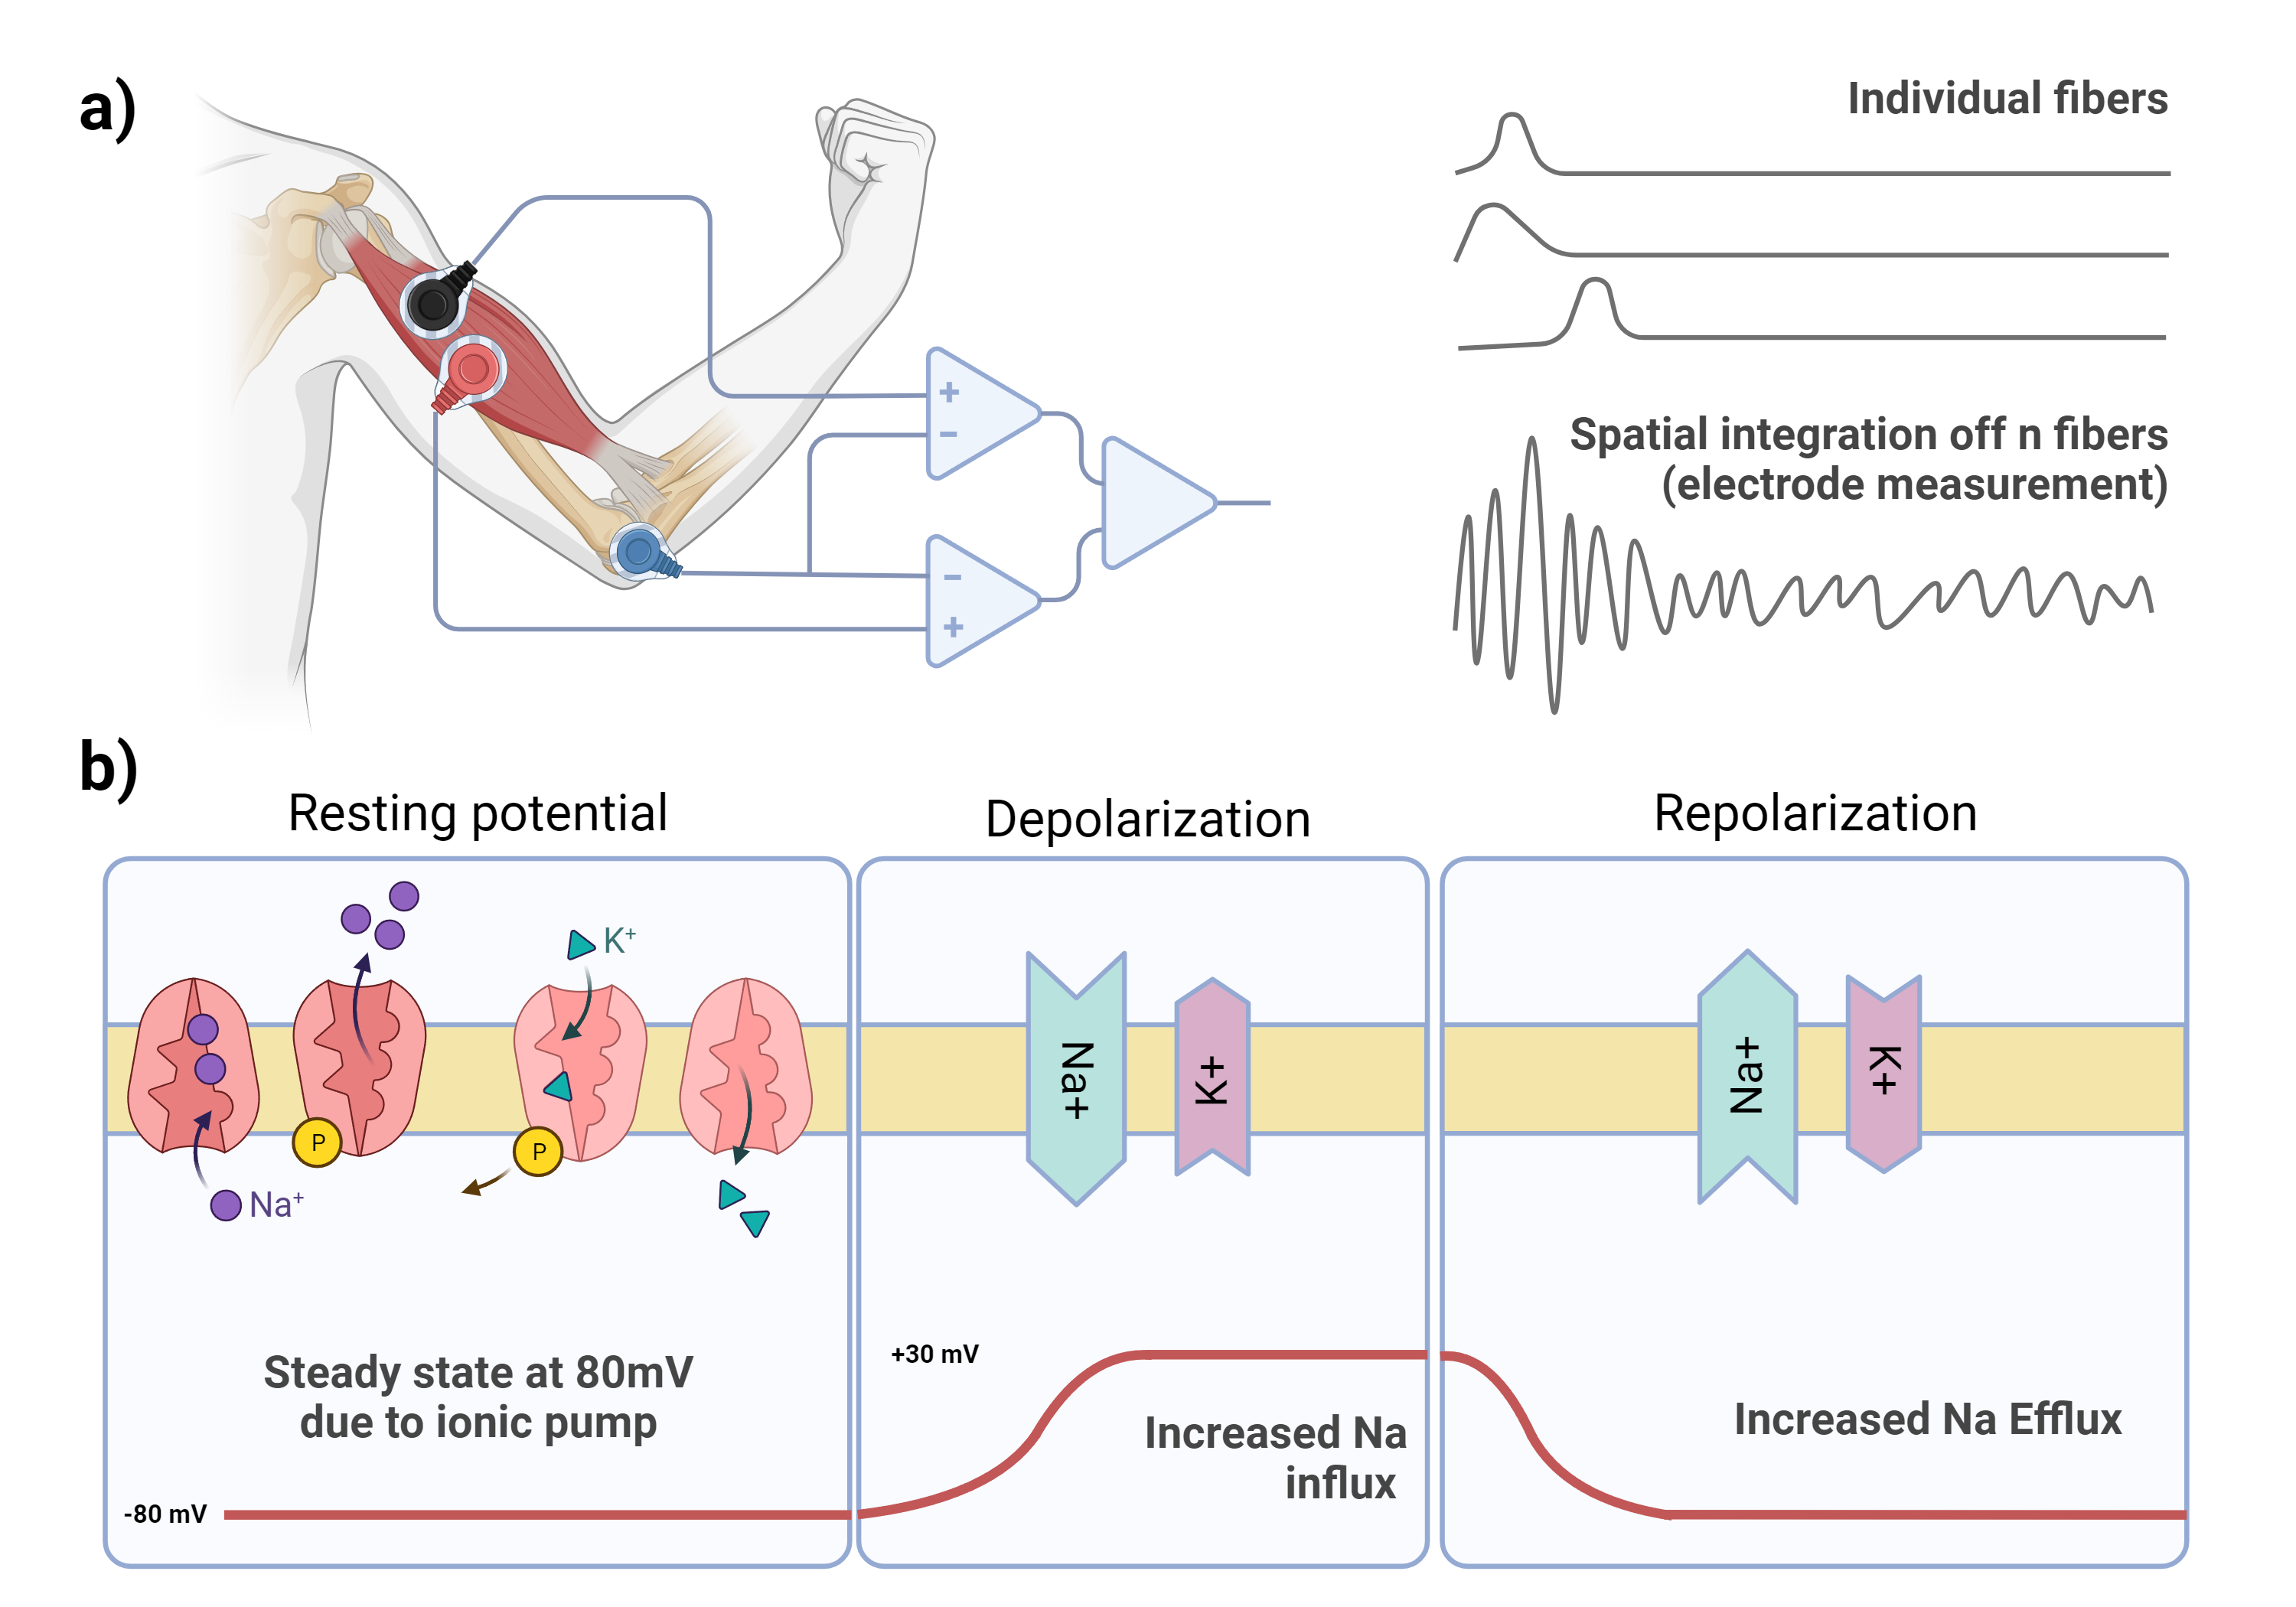
\includegraphics[width=1\linewidth]{actionpotential.png}
   \caption{Illustration of (a) electrode placement on a muscle for myoelectric signal monitoring, emphasizing the spatial resolution 
   challenge. Due to the electrode's size, significantly larger than individual muscle fibers, the detected signal integrates all fibers beneath the electrode. 
   (b) Diagram depicting the stages of a muscle cell's action potential, accentuating the ionic shifts during resting potential, depolarization, and repolarization.}
   \label{fig:actionpotential}
\end{figure}


\section{Materials and methods}
\subsection{Experiment set up and electrode positioning}

The electrodes were primarily positioned on the forearm, with the ground electrode 
placed on the hand, although variations were explored in some experiments. 

\begin{enumerate}
   \item \textbf{Subject Consistency:} 
   The experiments were conducted on a single individual to minimize the variance 
   typically associated with biological differences among different subjects.
   
   \item \textbf{Skin Preparation:} 
   The skin was cleaned using ethanol to remove any isolating layers such as fat 
   or other deposits, and allowed to air dry before electrode placement.
   
   \item \textbf{Electrode Type and Adherence:} 
   Generic Ag/AgCl (Silver/Silver Chloride) electrodes were used in this experiment. 
   They typically have a conductive gel embedded to enhance the 
   electrical connection between the skin and the electrode. The electrodes were adhered to the skin ensuring a snug fit for accurate sEMG 
   signal acquisition.
   
   \item \textbf{System Calibration:}
   The system was calibrated post electrode placement to ensure accurate capture 
   and display of the sEMG signals.
\end{enumerate}


\subsection{Signal processing and metrics}
\subsubsection{Signal normalization and segmentation}
Regarding \textbf{normalization}, initially, each signal was adjusted through a baseline correction, 
wherein the average value of the initial 500 milliseconds of the signal, where no action was performed (baseline period), was subtracted from the entire signal. 
This step aimed to correct any offsets or drifts in the data.  

In terms of \textbf{segmentation}, I adapted methodologies from a previous research \cite{wangResearchEMGSegmentation2019} into a Python code 
(Appendix 1.). Initially, the raw EMG data was processed to extract the envelope, which was subsequently utilized for segmentation purposes.
 This process entailed pinpointing the commencement and conclusion of muscle activations, relying on the derivative of the envelope and a predetermined 
 empirical threshold. To augment precision, these identified points were refined based on the integral of the envelope signal, including both the positive 
 and the negative counterparts. Furthermore, the segmented signals were time-normalized and overlaid for
 visual analysis, ensuring a consistent temporal scale across all segments (Figure \ref{fig:baselinecorrection}). 


\begin{figure}[h]
   \centering
   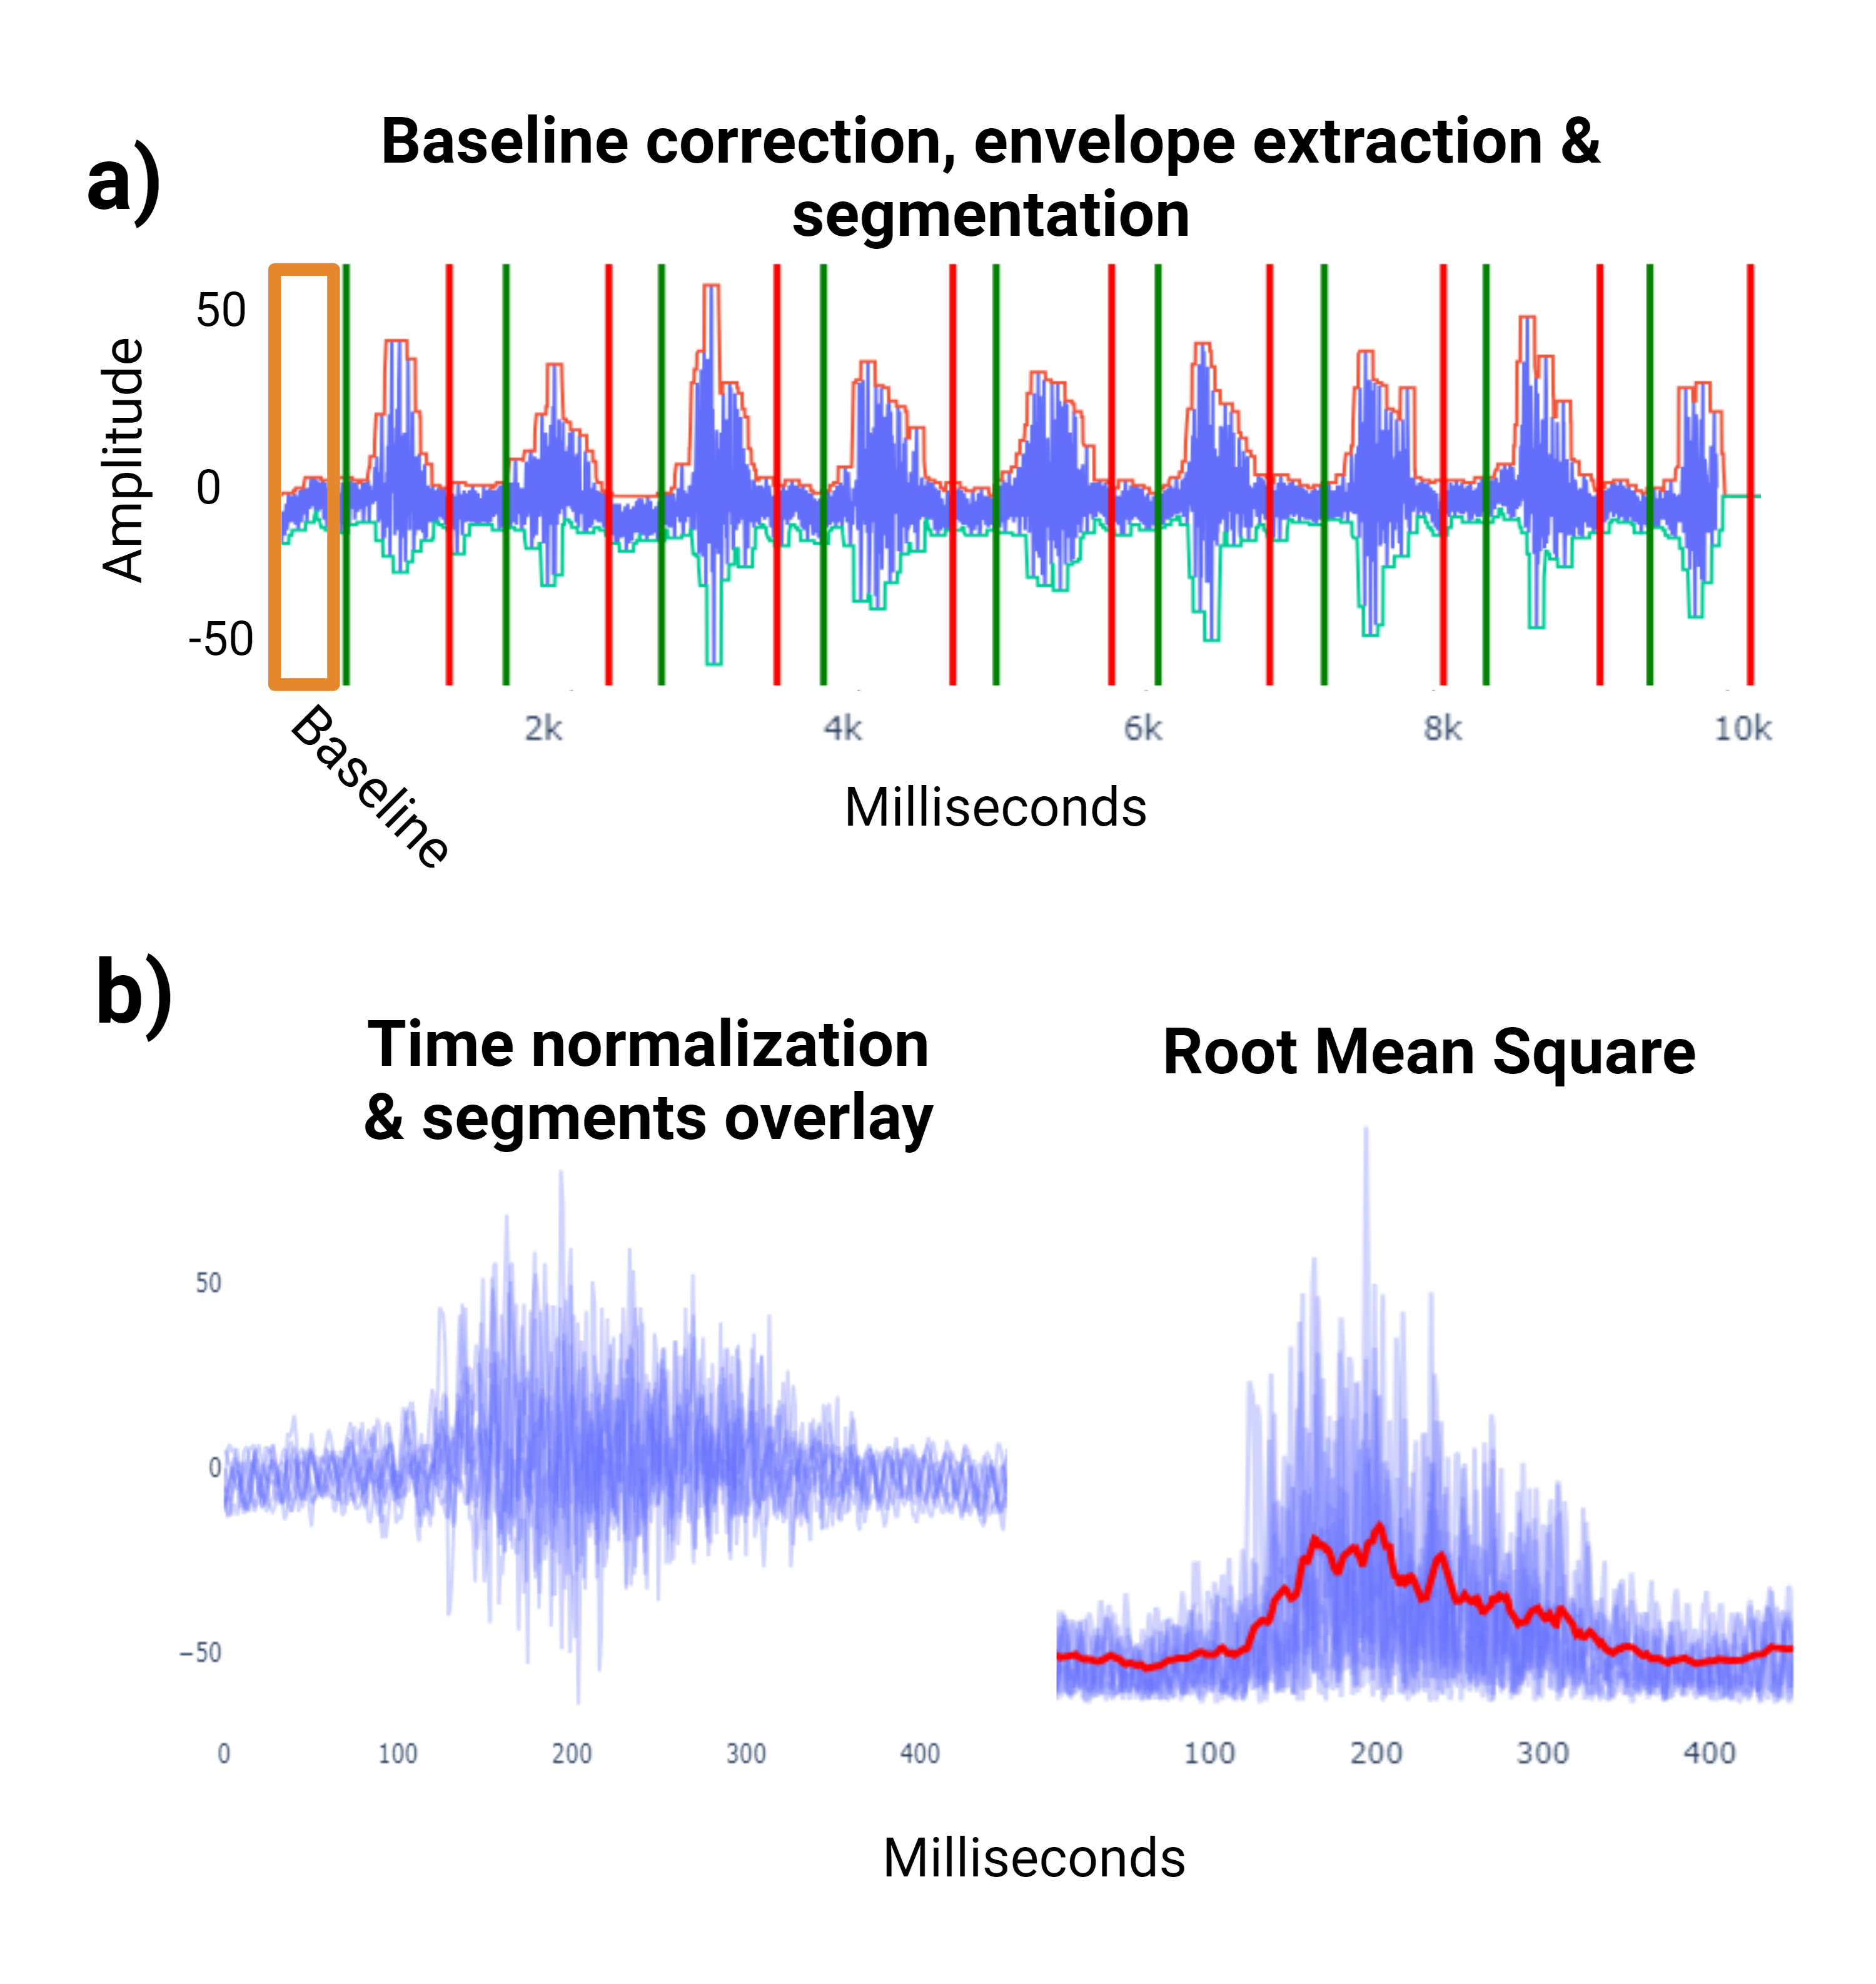
\includegraphics[width=1\linewidth]{baselinecorrection.png}
   \caption{Signal Processing Results: (a) Signal segmentation after baseline correction, envelope extranction and the subsequent segmentation 
   (b) Time normalization with segment overlay alongside Root Mean Square representation.}
   \label{fig:baselinecorrection}
\end{figure}

\subsubsection{Time domain analysis}
In my time domain analysis, I focused on analyzing the characteristics of the Root Mean Square graph and calculating the signal-to-noise ratio value for each condition.

To compute the \textbf{Root Mean Square (RMS)}, the individual segments (for data with only one repetition) or time-normalized segments were subjected to the following formula:

\[
\text{RMS}(t) = \sqrt{\frac{1}{N} \sum_{i=1}^{N} x(t_i)^2}
\]

where:
\begin{itemize}
    \item \( \text{RMS}(t) \) represents the root mean square value at time \( t \).
    \item \( N \) is the number of samples within the RMS window (chosen to be 10-milliseconds for this experiment), determined by the product of the window size and the sampling rate of the signal.
    \item \( x(t_i) \) denotes the signal value at the specific time point \( t_i \) within the window.
    \item \( t_i \) varies across each discrete time point in the window, capturing the fluctuations of the signal within that timeframe.
\end{itemize}

To assess the quality of the signal, I calculated the \textbf{Signal-to-Noise Ratio (SNR)} based on the power of the signal and the power of the baseline noise. 
The baseline noise was determined from the power of the signal during the initial 500ms of each experiment (As shown in figure \ref{fig:baselinecorrection}). 
The power of the signal and the baseline noise were calculated using the following equations:

\[
\text{Power of Signal} = \frac{1}{N} \sum_{i=1}^{N} \text{signal}[i]^2
\]

\[
\text{Power of Baseline Noise} = \frac{1}{M} \sum_{j=1}^{M} \text{noise}[j]^2
\]

The SNR was then calculated using the formula:

\[
\text{SNR (dB)} = 10 \cdot \log_{10}\left(\frac{\text{Power of Signal}}{\text{Power of Baseline Noise}}\right)
\]

This methodology provides a quantitative measure of the signal quality, aiding in the interpretation of the RMS graph and ensuring the reliability of the time domain 
analysis.

\subsubsection{Frequency domain analysis}
In the frequency domain analysis, my primary objective was to obtain the Total Power 
Spectrum (TPS) of the signal, which provides a comprehensive illustration of the signal's 
frequency content. The Fast Fourier Transform (FFT) was employed to transition from the time 
domain to the frequency domain, thereby enabling the computation of the TPS.

The procedure for obtaining the TPS is delineated below:

\begin{enumerate}
    \item \textbf{Preparation of Signal:} Initially, any NaN values in the signal were 
    handled by either interpolation or zero-filling to ensure a continuous dataset. Then the values were normalize by baseline correction (as explained previously).
    
    \item \textbf{Fast Fourier Transform (FFT):} The FFT was applied to the signal to 
    obtain the spectrum, utilizing the formula:
    \[
    X(f) = \sum_{n=0}^{N-1} x(n) \cdot e^{-j(2\pi/N) \cdot f \cdot n}
    \]
    where:
    \begin{itemize}
        \item \( X(f) \) denotes the FFT of the signal at frequency \( f \).
        \item \( N \) is the total number of samples.
        \item \( x(n) \) represents the signal value at sample \( n \).
        \item \( f \) is the frequency index ranging from 0 to \( N-1 \).
        \item \( j \) is the imaginary unit.
    \end{itemize}
    
    \item \textbf{Filtering:} An analysis without filtering was conducted on the raw signal,
    which resulted in prominent 50Hz peaks, highlighting significant noise caused by the power grid.
    Therefore, I established two filters: one filtering out the signals below 10Hz (associated with
    experimental repetitions), and another filtering out the signals between 49 and 51 Hz. The 50Hz filter was just 
    applied for plotting the FFT analysis, while the original signal was not altered. The time-domain analysis were, threfore,
    performed without the 50Hz filtering, because it would be difficult to discriminate which part of the signal comes from the power net and which is part of 
    the muscle, risking to delete part of the original signal filtering the entire 50Hz data.

    
\end{enumerate}

An illustrative representation of the FFT with and without filtering is depicted in Figure 
\ref{fig:fft_tps}.

\begin{figure}[h]
   \centering
   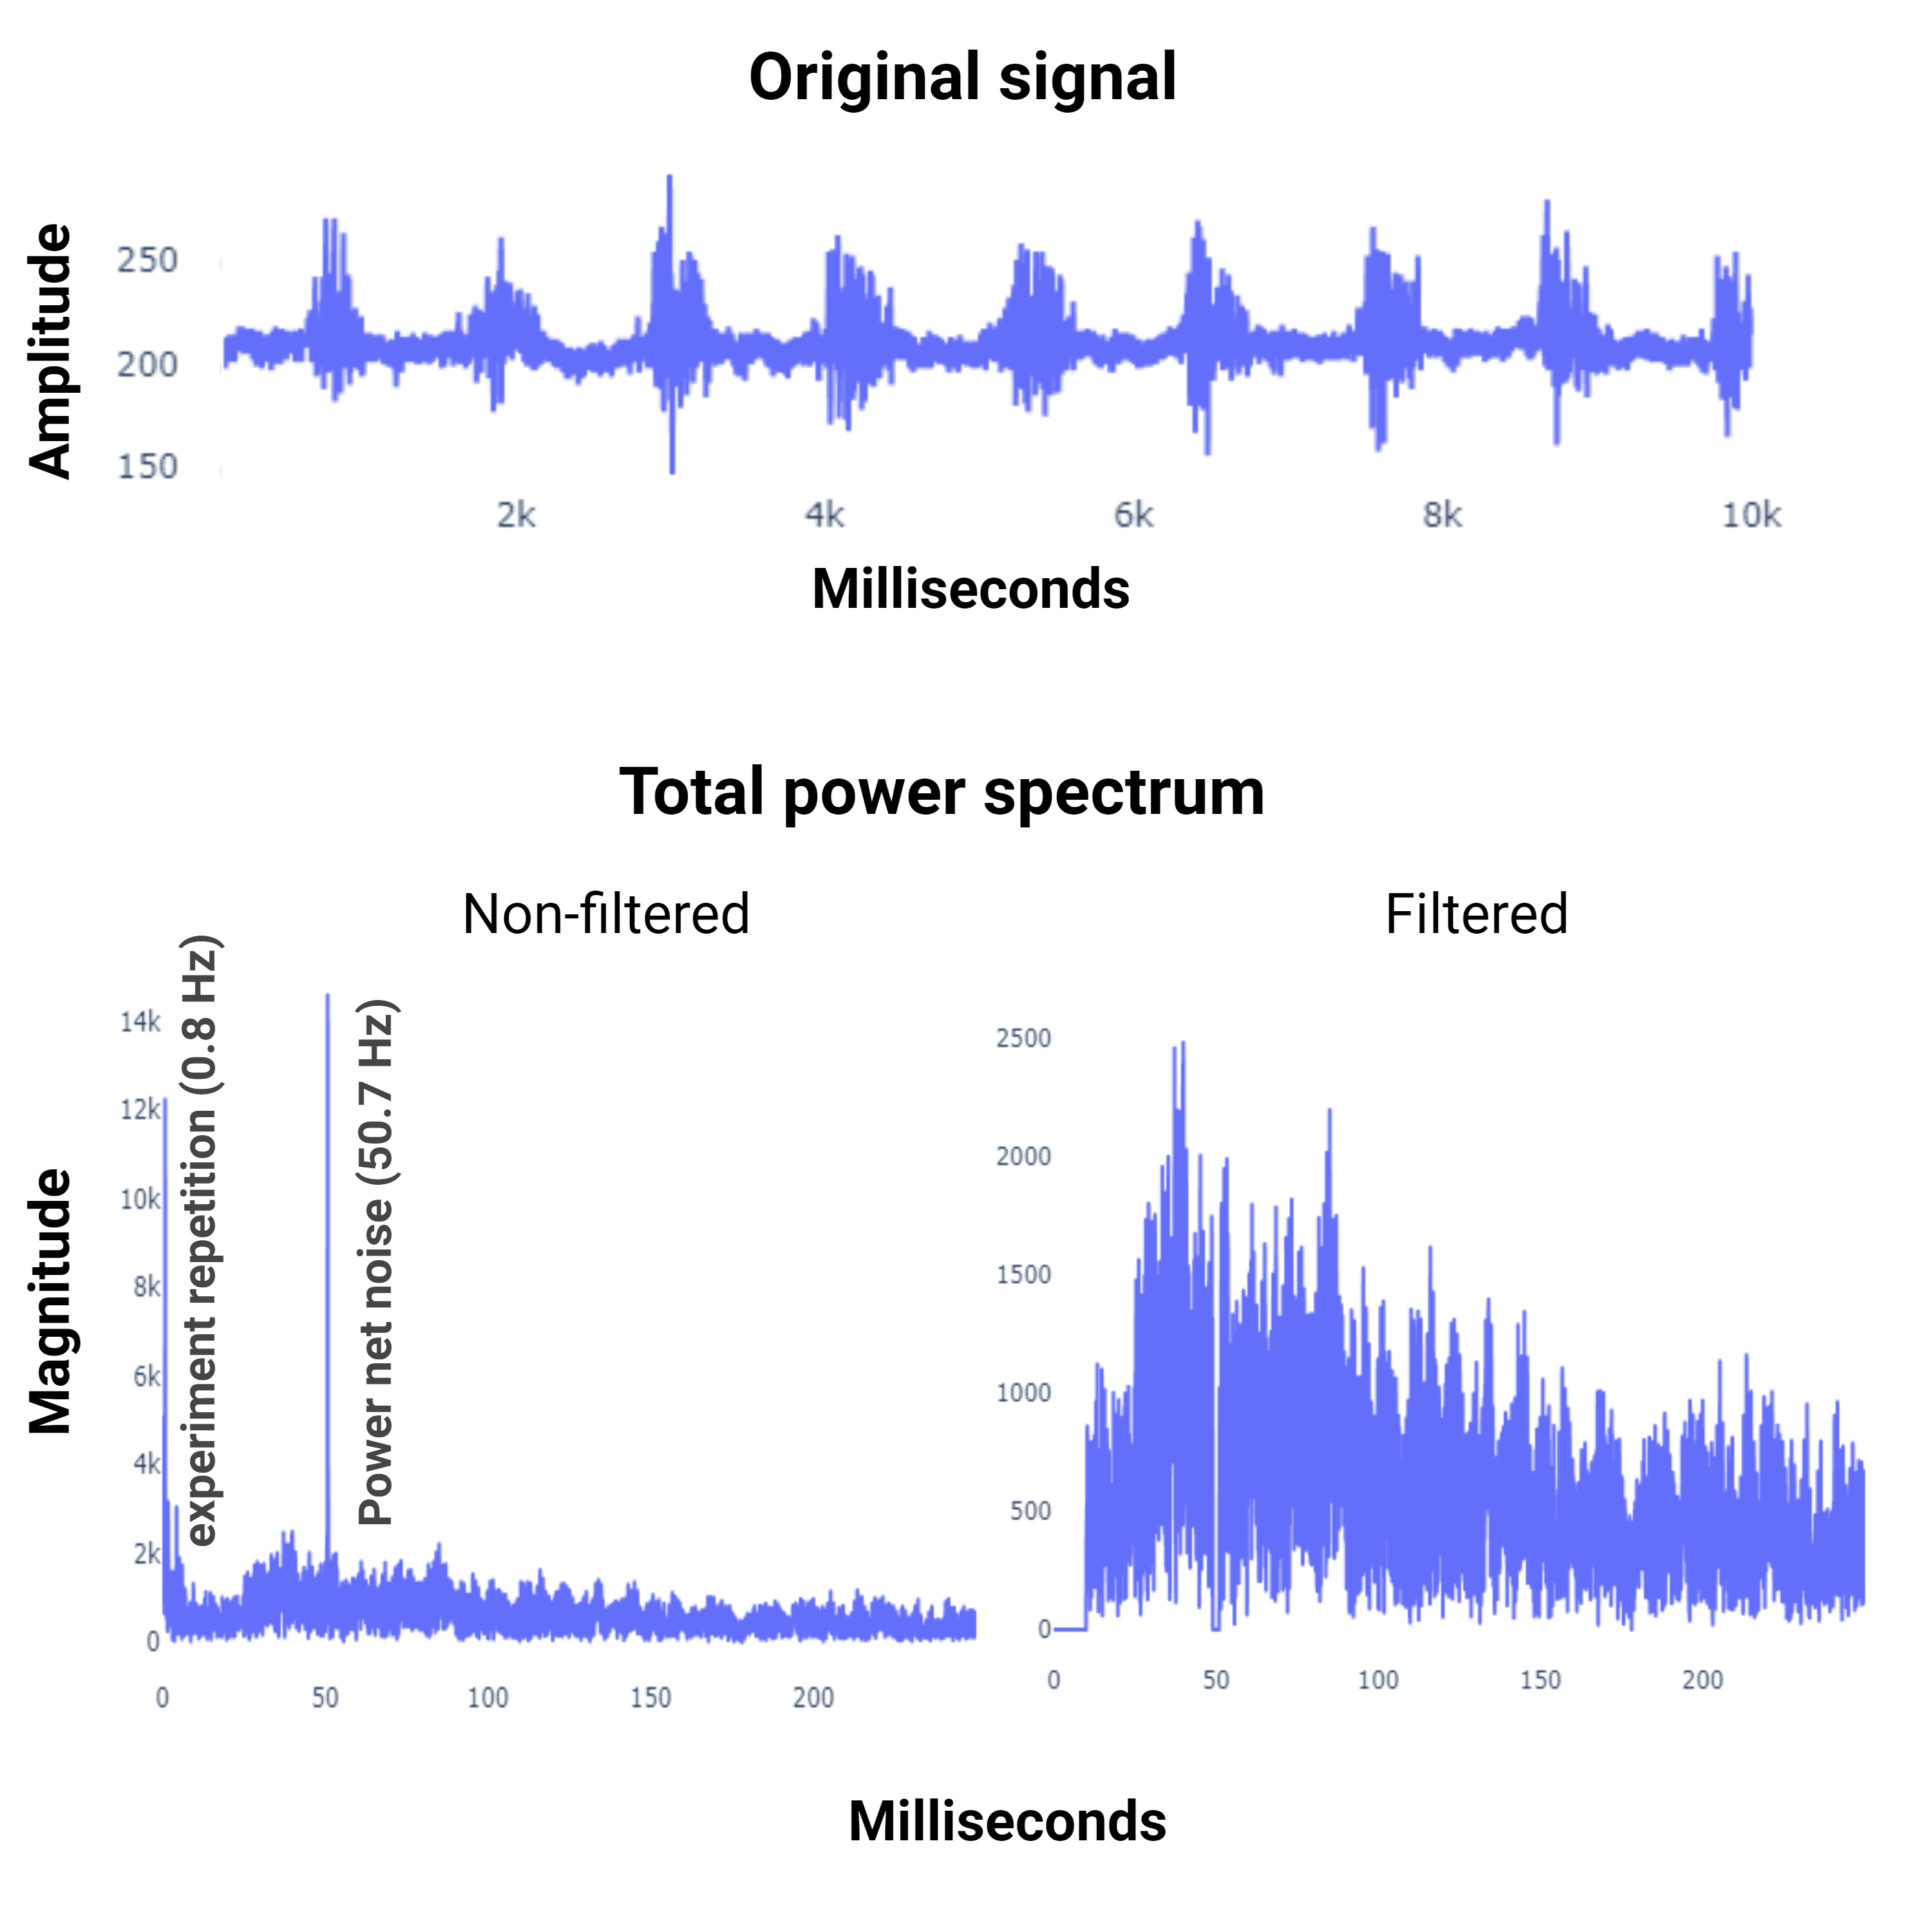
\includegraphics[width=1\linewidth]{fft_tps.png}
   \caption{Frequency Domain Analysis (FFT) before and after the 10 to 500 Hz filter but also removing the power net noise of 50Hz 
   (only for plotting, original signal not altered for other analysis).}
   \label{fig:fft_tps}
\end{figure}


\section{Results and discussions}

\subsection{Dependence of EMG recordings on experimental configuration}

\subsubsection{Electrode Location and Its Effects}

Previous research has often advocated for a parallel electrode 
disposition in sEMG, as it tends to 
align with the long axis of the muscle fibers, facilitating 
optimal signal collection \cite{youngEffectsElectrodeSize2011}.
However, a different study shows that when the EMG amplitude values were normalized, there 
were no significant mean differences observed between the two 
orientations, suggesting that the normalization process could 
equalize the values derived from both orientations \cite{zunigaEffectsParallelPerpendicular2010}.

Surprisingly, in our experiments, the perpendicular disposition 
exhibited a better amplitude in the RMS 
curve and an improved SNR ratio (Figure \ref{fig:parallelperp}). 
However, a potential cause could be explained after analyzing the frequency data. 
The parallel experiment displayed a power net (50Hz) signal peak 
that was twice as pronounced as that in the perpendicular 
experiment, indicating that the reduced SNR ratio in 
the parallel disposition might not stem from a decrease in the 
signal per se, but rather from an increase in noise, possibly 
due to inadequate insulation from the power net.

Interestingly, after filtering out the 50Hz noise, the 
perpendicular disposition showcased a more substantial signal 
presence at lower frequencies, potentially indicating the 
cross-talk from adjacent muscles that is associated by previous research 
with those frequencies (among other possibilities) \cite{germerSurfaceEMGCross2021}. 

\begin{figure}[h]
   \centering
   \includegraphics[width=1\linewidth]{parallelperp.png}
   \caption{Comparison of parallel vs perpendicular electrode disposition. The frequency analysis reveals
   how the power net related noise was much more prominent in the parallel configuration (\textcolor{myred}{red bracket}) than in the perpendicular one (\textcolor{myblue}{blue bracket}).
   Another interesting result from the frequency analysis is the higher presence of low frequency signal in the perpendicular configuration (\textcolor{mygrey}{grey box}) that 
   is described to be an indicator of cross-talk (among other origins) \cite{germerSurfaceEMGCross2021}.}
   \label{fig:parallelperp}
\end{figure}

\subsubsection{Electrode Size and Its Impact}
The second experiment, which involved masking part of the electrode 
with paper, highlighted the significant influence of electrode 
size on sEMG recordings. Both the raw signal and the time normalized RMS
rom the masked electrodes exhibited more distinct and pointed peaks compared 
to the non-masked setup, likely due to reduced spatial 
integration stemming from the smaller electrode surface area. 
This reduced surface area leads to capturing signals from fewer 
muscle fibers, rendering the readings more localized and 
specific (Figure \ref{fig:masked}). 

Regarding to the noise distribution on both signals,
the baseline noise was observed to be wider for the masked 
electrodes, and at the same time, the SNR Ratio was considerably lower (0.68) compared to the non-masked 
electrodes (5.73). Both these metrics reflect an increase of noise 
in the masked electrode vs the full area one. One possible cause 
might be the reduced surface area of the masked electrodes, 
which could make them more sensitive to local, minute 
fluctuations. Another potential factor that may be affecting the 
noise increase is a potential increase in impedance (due to the 
paper masking and the subsequent contact surface reduction), further contributing to the 
broader noise baseline observed. These factors could also 
explain the behavior observed in the total power spectrum, 
where the frequency distribution in the masked 
setup remained relatively consistent, while the non-masked setup 
showed more variability. This variability in the non-masked 
setup might be due to the broader noise dispersing the energy 
across the spectrum, rendering distinct peaks (The signal) less noticeable.

In summary, the non-masked electrodes offered a clearer and more 
generalized signal by capturing inputs from a broader muscle 
fiber range, thus providing a higher SNR and more defined peaks. 
Conversely, the masked electrodes, with their limited surface 
area, produced more localized and punctual peaks, although at 
the cost of a broader noise baseline. These observations underscore the 
role that the design and size of the electrodes play in the 
type of muscle fiber signals they capture, and consequently, 
the quality of the resultant data. The findings align with 
existing literature that electrode size, including surface 
area, is a crucial parameter in sEMG measurements, impacting 
signal quality, noise levels, and the representativeness of the 
captured muscle activity \cite{hermensDevelopmentRecommendationsSEMG2000,merlettiTutorialSurfaceEMG2020}.

\begin{figure}[t]
   \centering
   \includegraphics[width=1\linewidth]{masked.png}
   \caption{Comparison of full area vs reduced-area electrode signal.}
   \label{fig:masked}
\end{figure}

\subsection{Processing of EMG recordings}
A straightforward method to convert the raw EMG recordings 
measured at different flexion forces into a signal to drive a 
motor of a prosthetic arm would involve several processing steps,
all of them computationally light, so the signal can be mapped to a motor action in real time. The steps are as follows:

\begin{itemize}
   \item \textbf{Filtering:} Initially, the algorithm would apply a band-pass filter to the 
   raw EMG data to isolate the frequency range of 20 to 500 Hz, 
   which corresponds to the frequency range of muscle contractions. 
   To mitigate the power net parasitic signals previously mentioned, 
   a 50Hz notch filter should be applied to reduce the power supply noise.
   
   \item \textbf{Rectification and Smoothing:} Following filtering, 
   a simple method to rectify, smooth, and average the signal would be 
   calculating the RMS of the signal over a moving window (determined based on the muscle/patient).
   Then, calculate the delta of the EMG signal from the baseline (\( \Delta S \)) by subtracting the baseline value from the RMS (Figure \ref{fig:prothesis} (top)).
   
   \item \textbf{Thresholding:} The next step would involve setting up a threshold that allows to proceed with 
   the subsequent mapping only when a muscle activation is detected. To do so, a 
   pre-calibration phase would be necessary to study the shape of the baseline noise 
   and the activation signal.
   
   \item \textbf{Mapping to Motor Control:} Lastly, it would be necessary to map the processed 
   EMG signal to the motor control input of the prosthetic arm. 
   For instance, if the processed EMG signal value is 0.5, and the 
   motor operates at a speed range of 0 to 100 RPM, the motor 
   speed could be set to 50 RPM (i.e., 0.5 * 100). This mapping 
   could be linear or non-linear depending on the design 
   requirements, and should be tuned to ensure a responsive and 
   intuitive control for the user (Figure \ref{fig:prothesis} (bottom)).
\end{itemize}


\begin{figure}[h]
   \centering
   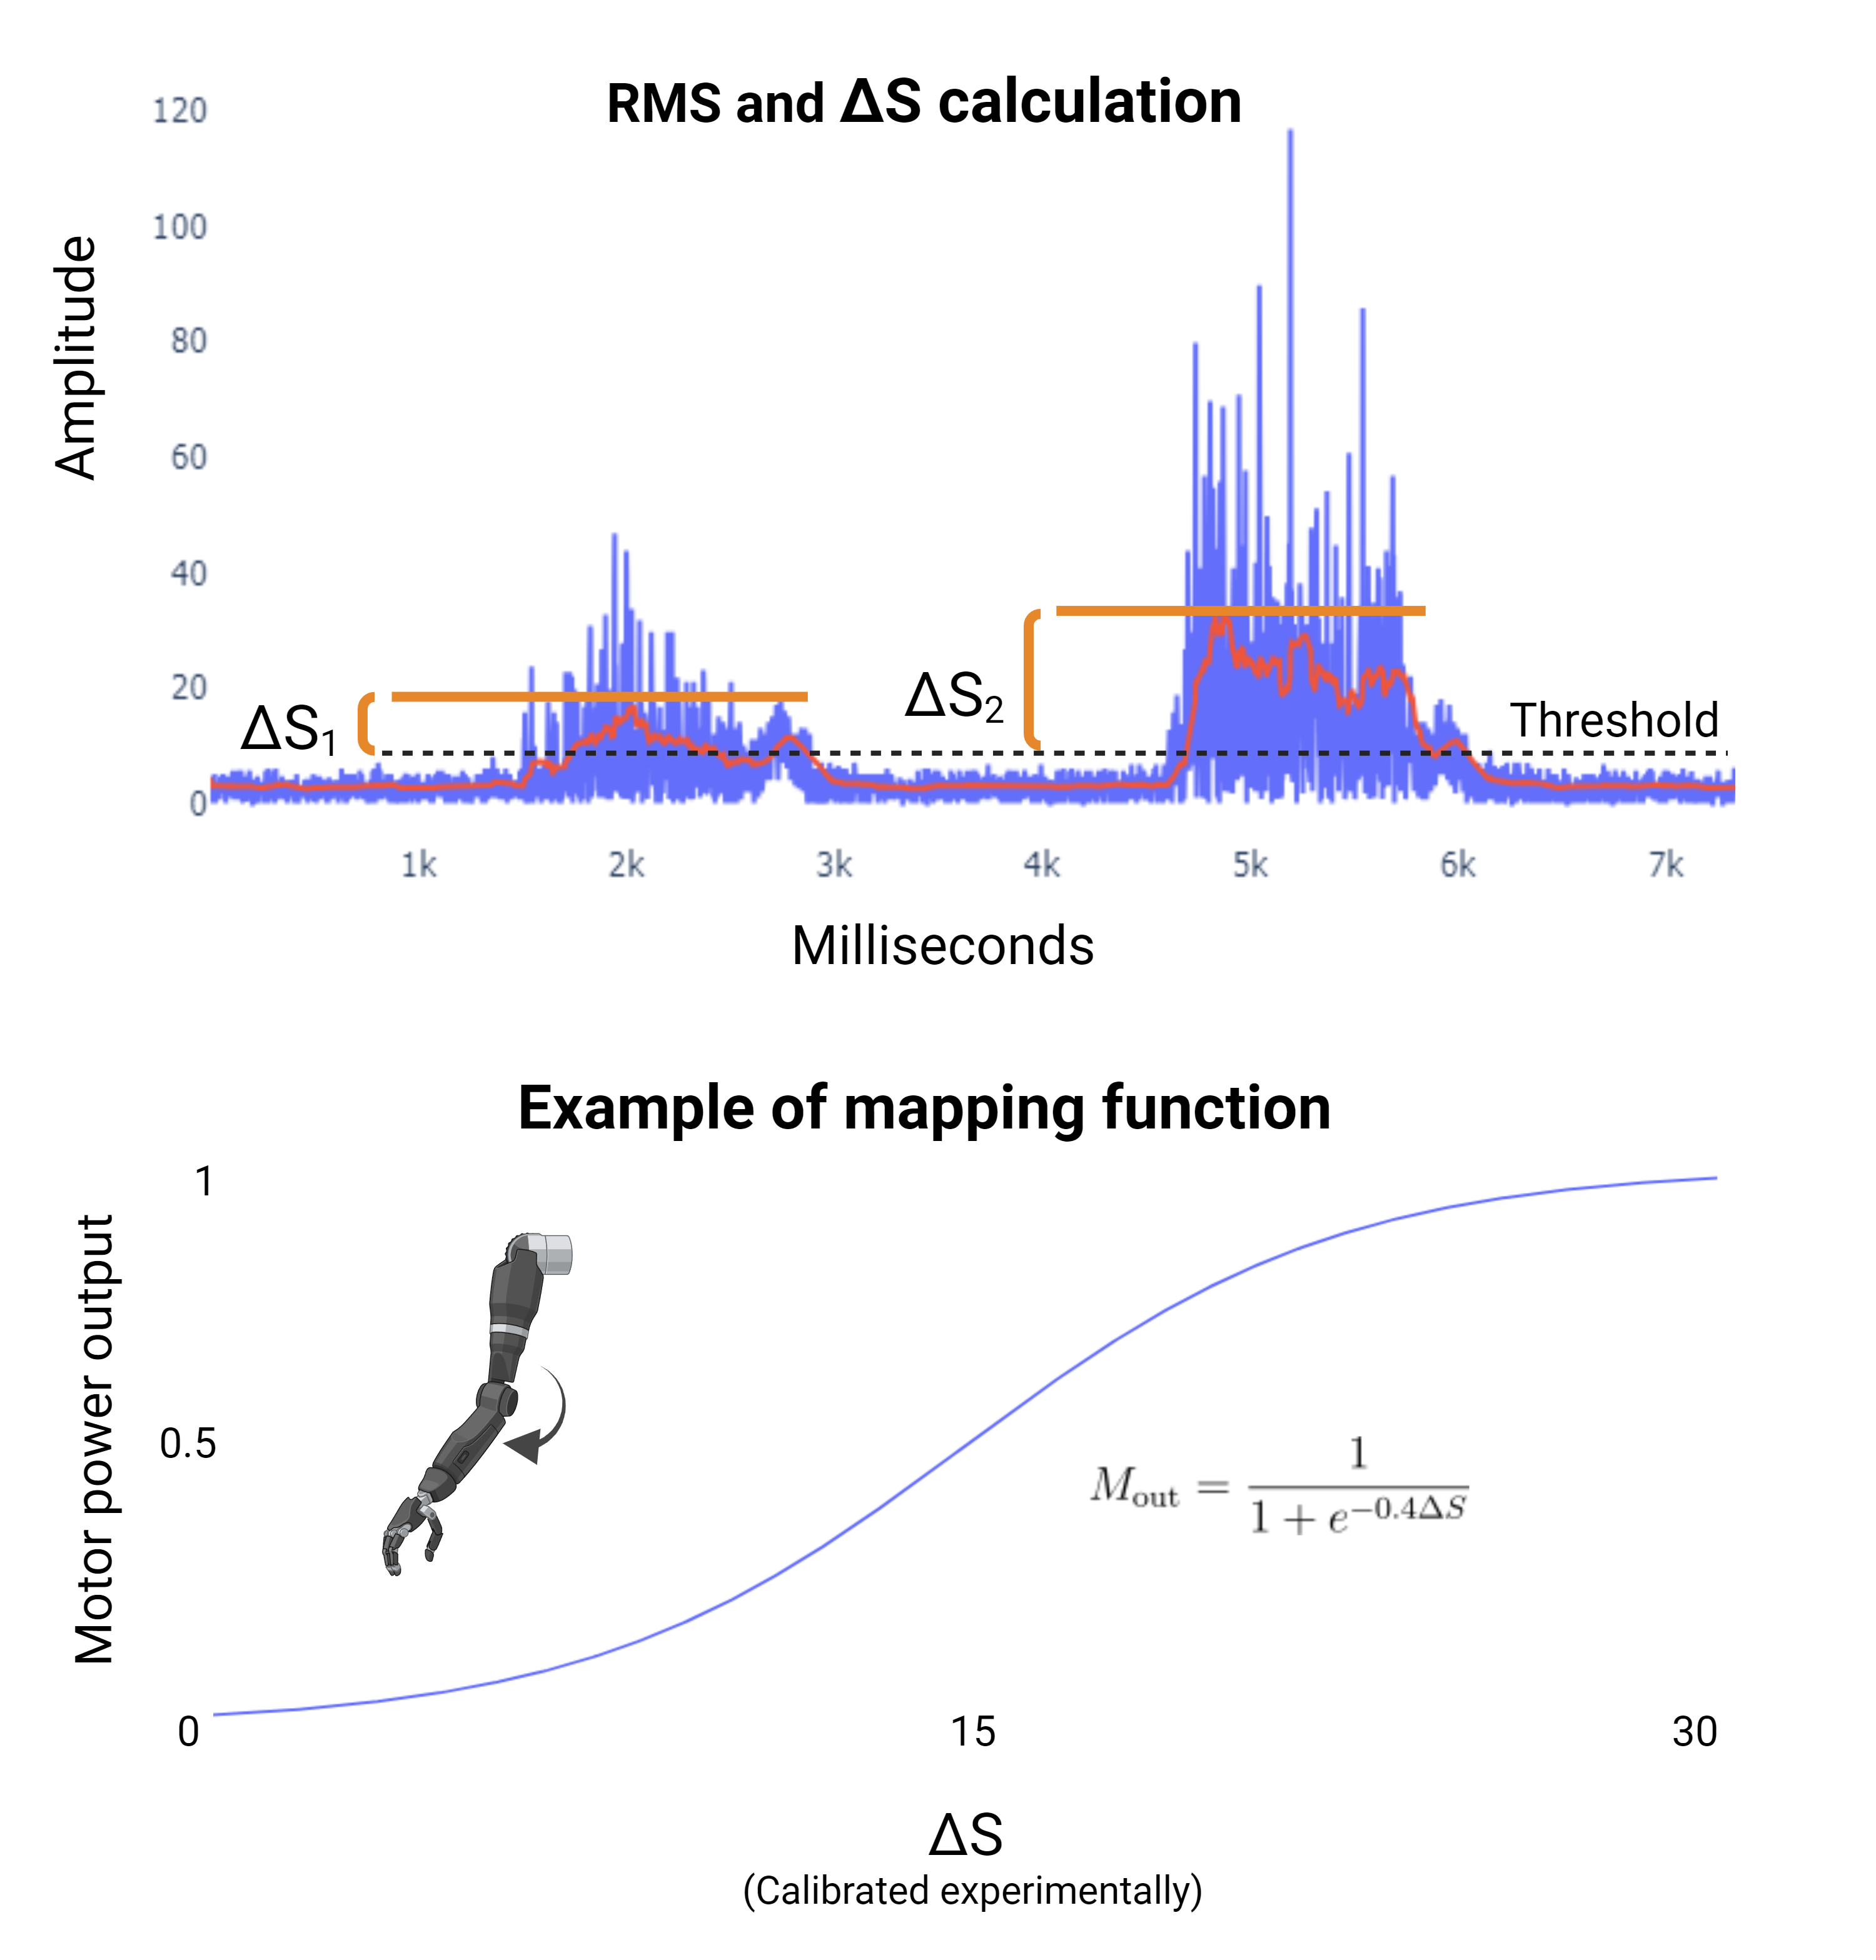
\includegraphics[width=1\linewidth]{prothesis movement.png}
   \caption{(Top) Representation of the sEMG signal illustrating RMS values and the calculated (\( \Delta S \)) intervals above a set threshold. The two peaks correspond to a weak and a strong
   muscle activation (from left to right). (Bottom) Example of a sigmoideal mapping function showcasing the relationship between (\( \Delta S \)) values and the corresponding motor power output in a prosthetic device.}
   \label{fig:prothesis}
\end{figure}

\subsection{Limitations of the EMG for prostheses}

\begin{itemize}
   \item \textbf{Resolution of Individual Muscle Activity:} 
   Large electrodes capture combined sEMG signals, obscuring the 
   activities of individual muscles during finer movements like finger motions. 
   The overlapping signals make it difficult to achieve precise control 
   over prosthetic devices. The lack of spatial resolution hinders the 
   differentiation of signals from individual muscle fibers, impacting 
   the accuracy of prosthetic control.


   \item \textbf{Force Discrimination:}
   The ability to discriminate different levels of flexion force largely 
   depends on a good SNR ratio. When the force exerted is subtle, 
   the resulting sEMG signal may be smaller than the noise level, making it 
   indistinguishable. This limitation also establishes the limit of granularity in the ability
   to distinguish between two forces.
   
   
   \item \textbf{Muscle Fatigue:} 
   Prolonged usage or repetitive motions may lead to muscle fatigue, 
   which could alter the sEMG signal characteristics (As varying the correlation amplitude-force), 
   affecting the control accuracy over time.
   
   \item \textbf{Calibration:}
   \begin{itemize}
       \item The sEMG signal profiles and noise levels may vary among 
       different individuals, necessitating personalized calibration for 
       optimal performance.
       \item Frequent recalibrations might be needed to maintain accurate 
       control, especially in long-term or continuous usage scenarios 
       (where also muscle fatigue or body conductivity start playing an important role).
       \item In some instances, such as in the experimental conditions, the sEMG noise levels 
       changed significantly within a short period (due to external changes in the power supply isolation)
       , indicating a need for adaptive calibration strategies.
   \end{itemize}
   
   \item \textbf{Same Profile Signal:} 
   A robust finger movement and a mild arm flexion may generate sEMG 
   signals of similar amplitude, posing challenges for accurately mapping 
   sEMG signals to intended motor actions.
\end{itemize}

\section{Conclusions}

This practice has taught me a lot about the capabilities and limitations of the sEMG technique, 
as well as what it needs to be improved. The unexpected results from the experiment comparing parallel and 
perpendicular electrodes (Figure \ref{fig:parallelperp}), which were different from what other studies have found, highlight the 
importance of having an internal check on data quality. In particular, the fact that in one of the experiments 
the 50Hz noise signal was more than twice as strong clearly (And the particularly contradicting conclusions that the experiment results could led to take) 
shows the risks of compararing two signals without internal data controls. For future work, a way to avoid this risks could consist in running a quick 
check after the experiment to make sure the 50Hz noise is the same in all the data sets. This will reveal which experiments have too much 
noise, enabling the researchers to repeat them on time.

On the flip side, the experiments with varying electrode sizes (Figure \ref{fig:masked}) taught me about the trade-off between 
spatial resolution and signal quality. As the size of the electrode was reduced, it was noticed an increase 
in spatial resolution but a decrease in signal quality, partly due to a rise in impedance. Finding the right 
balance between these two factors is crucial, and it involves careful calibration and the use of processing 
algorithms that can enhance the signal in real-time without causing any delays.

In addition, while the results of experiments on single finger movements are not shown (due to 
the already long report dimension), the observations made it clear that using just two electrodes is not sufficient for 
capturing detailed information to distinguish between complex movements, such as the movement of different
 fingers. For more advanced applications, like controlling prosthetic hands with precision, it would be 
 beneficial to use a combination of larger and smaller electrodes. The smaller electrodes would provide the 
 high spatial resolution needed to pick up on subtle movements, while the larger ones would ensure the signal
  quality is maintained.

\bibliographystyle{IEEEtran}
\bibliography{biosensors_class.bib}
\vspace{2cm}
\section{Compliance}
\wordcount / Total figures: \thetotalfigures\vspace{0.2cm}
\break
\small{Words calculated automatically using texcount package (https://app.uio.no/ifi/texcount/) on the original LaTeX file (bibliography not included).}

\end{document}
